\chapter{\drexstitle: single mantle aggregate LPO fabrics with D-Rex}
\label{chapter:drexs}

\drexstitle{} is a software that is designed for testing the evolution of mantle fabrics and related elastic properties of a single aggregate, as a function of the flow field, amount of strain, crystal plasticity, P-T conditions and SPO fabrics. It builds on the original \textbf{D-Rex} software \citep{kaminski2004gji}.\\
Five different types of 2-phases mantle aggregates, hereafter named rocktypes, are available:\\ 
\vspace{0.1cm}


\fonts{1} = Ol:Ens, for the upper mantle (UM: 0-410 km)\\ 
\fonts{2} = Wd:Grt, for the upper transition zone (UTZ: 410-520 km)\\ 
\fonts{3} = Rw:Grt, for the lower transition zone (LTZ: 520-660 km)\\ 
\fonts{4} = Brd:MgO, for the lower mantle (LM: 660-2900 km)\\ 
\fonts{5} = pPv:MgO, for the bottom of the lower mantle\\ 

The LPO evolution is computed for Olivine, Enstatite, Wadsleyite, Bridgmanite and post-Perovskite, while other major phases such as Garnet, Ringwoodite and MgO are considered to be isotropic and their distribution is set to random.
Thus, no LPO is computed for rocktype \fonts{3}, and anisotropy in the LTZ arises only when SPO modeling is active.\\

The fabrics generated with \drexstitle{} can also be used to impose pre-existing microstructures on multiple crystal aggregates lying within a specific subdomain of large scale geodynamic models. The computed final LPO and F\textsubscript{ij} are saved to \texttt{fossilfabric.h5}, and can be subsequently loaded during the \drexmtitle{} simulations upon setting \fonts{fossilfabric} > 0 in \texttt{drexm\_input.dat} (see section \ref{section:modelsetup}).
\vspace{0.5cm}

\texttt{COMPILE: ./bash\_compile}\\*

\texttt{RUN: ./drexs drexs\_input.dat}\\*


\section{Parameter input file}

The following information need to be set in the parameter input file \texttt{drexs\_input.dat} (unless otherwise specified, the variable format is FORTRAN \texttt{double precision}):

A) Output file/directory name
\begin{itemize}
    \item \fonts{output\_name}: (String) if not existing, a new directory is created with output files saved each $0.1$ strain increment. The output files are named as\\ \texttt{[\fonts{output\_name}]+[strain]+[.h5]} (example: if \fonts{output\_name} = \texttt{UM\_},\\ \fonts{strain\_max} = 1.0, the output files will be \texttt{UM\_0.1.h5}, \texttt{UM\_0.2.h5}, \ldots, \texttt{UM\_1.0.h5}). When \fonts{spomod} > 0, an additional output file is generated at the end of the run named as \texttt{[\fonts{output\_name}]+[SPO.h5]} (example: \texttt{UM\_SPO.h5}).
\end{itemize}
\vspace{0.5cm}

B) Maximum strain
\begin{itemize}
    \item \fonts{strain\_max}
\end{itemize}
\vspace{0.5cm}

C) Velocity gradient tensor D\textsubscript{ij}
\begin{itemize}
    \item \fonts{D\textsubscript{11},...,D\textsubscript{32}}: components of the velocity gradient tensor
    
\end{itemize}
\vspace{0.5cm}

D) LPO parameters:
\begin{itemize}
    \item \fonts{size3}: (Integer) cubic root of total number of grains in the aggregate for each of the 2 mineral phases (e.g.: \fonts{size3} = 10 $\rightarrow$ 1000 crystals of phase 1 and 1000 crystals of phase 2). 
    \item \fonts{rocktype}: (Integer) define the mantle aggregate (\fonts{1},\fonts{2},\fonts{3},\fonts{4},\fonts{5})
\end{itemize}
\vspace{0.5cm}

\hspace{0.5cm} For each of the 5 different types of aggregate\footnotemark:
\vspace{0.5cm}

\footnotetext{Rw and Grt are assumed to be isotropic at MTZ depths, and therefore no LPO is computed for this aggregate. Consequently, only \fonts{Xol} and \fonts{single\_crystal\_elastic\_db} need to be set.}

\begin{itemize}
    \item \fonts{Xol}: volume fraction of Ol, Wd, Rw, Brd, pPv (in \%)
    \item \fonts{stressexp}: stress exponent for non-Newtonian plasticity  
    \item \fonts{Mob}: efficiency of grain boundary migration 
    \item \fonts{chi ($\pmb{\chi}$)}: volume fraction threshold below which no dislocation creep occurs   :e
    \item \fonts{lambda ($\pmb{\lambda}$)}: efficiency of grain nucleation
    \item \fonts{fractdislrock}: fraction of deformation accommodated by the anisotropic phase
    \item \fonts{tau1...tauN}: normalized CRSS of the anisotropic phase slip systems. For upper mantle aggregates (rocktype = 1), tau(1,1-4) are for olivine, while tau(1,5)=1 is for enstatite. See \ref{table:1}.
    \item \fonts{single\_crystal\_elastic\_db}: (Integer) choose single crystal elastic tensor for phase 1 and 2 from those compiled in elastic\_database.f90. See \ref{table:2}.
\end{itemize}

\vspace{1cm}

E) Operating modes:
\begin{itemize}

    \item \fonts{ptmod}: (Integer)
    \begin{itemize}
        \item[] \fonts{0} = use single crystal tensors at room P-T conditions
        \item[] \fonts{1} = scale elastic moduli by local P-T conditions defined below
    \end{itemize}
    \item \fonts{eosmod}:  (Integer) set the domain lithology (\fonts{1}: Dunite; \fonts{2}: Harzburgite; \fonts{3}: Pyrolite; \fonts{4}: Basalt; \fonts{5}: Pyroxenite) for which the corresponding lookup tables of density, isotropic Vp and Vs computed with \mmaeostitle{} are loaded (see Table \ref{table:3}). The isotropic Vp and Vs are used to compute the isotropic component of the elastic tensor scaled at the local P-T conditions.
    \item \fonts{pressure}: pressure (in GPa)
    \item \fonts{tkelv}: temperature (in Kelvin)
    \item \fonts{fractvoigt}: fraction of Voigt averaging scheme when calculating the aggregate elastic tensor in \%. It varies from 0.0 (Reuss average) to 100.0 (Voigt average). When equal to 50.0, it yields the Hill average.
    
    \item \fonts{spomod}:  (Integer) when > 0, computes extrinsic elastic anisotropy\footnotemark{} saved in output file \texttt{[\fonts{output\_name}]+[SPO.h5]}
    \begin{itemize}
        \item[] \fonts{0} = no extrinsic elastic anisotropy
        \item[] \fonts{1} = extrinsic elastic anisotropy due to grain-scale or rock-scale layering (STILWE model)
        \item[] \fonts{2} = extrinsic elastic anisotropy due to the presence of aligned inclusions (DEM model)
        \item[] \fonts{3} = extrinsic elastic anisotropy due to the presence of aligned inclusions (DEM model) superimposed over the LPO fabric.
    \end{itemize}
\end{itemize}

\footnotetext{The SPO modeling is explained in detail in section \textbf{\ref{section:elasticSPO}}}

\section{Fabric visualization}
Fabric visualization requires the installation of the \texttt{MTEX toolbox} (\citet{mainprice2011gsl}). A recently tested version is 5.10.2, but previous versions 5.* should work as well. Please refer to the MTEX download webpage (\url{https://mtex-toolbox.github.io/download}) for installation instructions. 
\\
The aggregate fabric can be visualized with the \matlabtitle{} script \texttt{/viz/read\_Cij\_LPO.m} that allows to plot pole figures of the LPO, Vp, Vs1 and dVs, for multiple output files, which then can be combined into animations, together with the possibility to display the evolving fabric strength (M-index, J-index), anisotropy and its components (obtained with tensor decomposition; \citet{browaeys2004gji}) as a function of strain.
\\
The control parameters to be set in the first part of the script are (Fig. \ref{fig:drexs_viz}, Fig. \ref{fig:atype}, Fig. \ref{fig:miji}, Fig. \ref{fig:azirad}, Fig. \ref{fig:dec}):
\begin{itemize}
    \item \fonts{input\_dir}: (String) path to \drexstitle{} output files directory.
    \item \fonts{output\_dir}: (String) output directory where images and videos are saved.
    \item \fonts{fname0}: (String) first part of output file name (same as \fonts{output\_name} in \texttt{drexs\_input.dat}).
    \item \fonts{min\_strain}, \fonts{stp\_strain}, \fonts{max\_strain}: minimum, increment and maximum strain as indicated in the second part of the output file name to be visualized. When \fonts{min\_strain} = \fonts{max\_strain}, only a single output file is visualized.
    \item \fonts{plot\_Cij\_LPO}:  (Boolean) when true, activates plotting pole figures for Vp, dVs and LPOs. 
    
    \begin{itemize}
        \item \fonts{plot\_Voigt}:  (Boolean) when true, plot Vp, Vs1, dVs due to aggregate LPO, Voigt average.
        \item \fonts{plot\_Reuss}:  (Boolean) when true, plot Vp, Vs1, dVs due to aggregate LPO, Reuss average.
        \item \fonts{plot\_Mixed}:  (Boolean) when true, plot Vp, Vs1, dVs due to aggregate LPO, mixed Voigt/Reuss average as specified by \fonts{fractvoigt} in \texttt{drexs\_input.dat}.
        \item \fonts{plot\_Phase1LPO}: (Boolean) when true, plot LPO pole figures of main anisotropic phase, together with a plot of the M-index and J-index.
        \item \fonts{plot\_Phase2LPO}: (Boolean) when true, plot LPO pole figures of enstatite, together with a plot of the M-index and J-index (only for UM aggregates).
    \end{itemize} 
    
    \item \fonts{makevideo}: (Boolean) when true, generate animations of Vp, dVs and LPO pole figures evolution as specified by the 5 \fonts{plot\_*} operational modes defined above. 
    
    \item \fonts{plot\_azirad}: (Boolean) when true, plot azimuthal and radial P and S anisotropy, and $\eta$ parameter, as a function of strain for the tensors activated with \fonts{plot\_Voigt}, \fonts{plot\_Reuss}, \fonts{plot\_Mixed}.

    \item \fonts{plot\_dec}: (Boolean) when true, plot (i) the norm of the total anisotropy component of the tensor over the norm of the full tensor (in \%), and (ii) the norm of each anisotropic component of the tensor normalized over the norm of the total anisotropic component (in \%). These have been obtained by decomposition (\citet{browaeys2004gji} of the elastic tensor (Mixed average) and saved in file \texttt{anisdec.h5]}.
    
    \item \fonts{plot\_SPO}: (Boolean) when true, plot Vp, dVs due to SPO from the \texttt{[\fonts{output\_name}] +[SPO.h5]} output file.  
        
    \item \fonts{printmod}: (Boolean) when true, save images in \texttt{*.png} format.
\end{itemize}
\vspace{1.0cm}

\begin{figure}[ht]
    \centering
    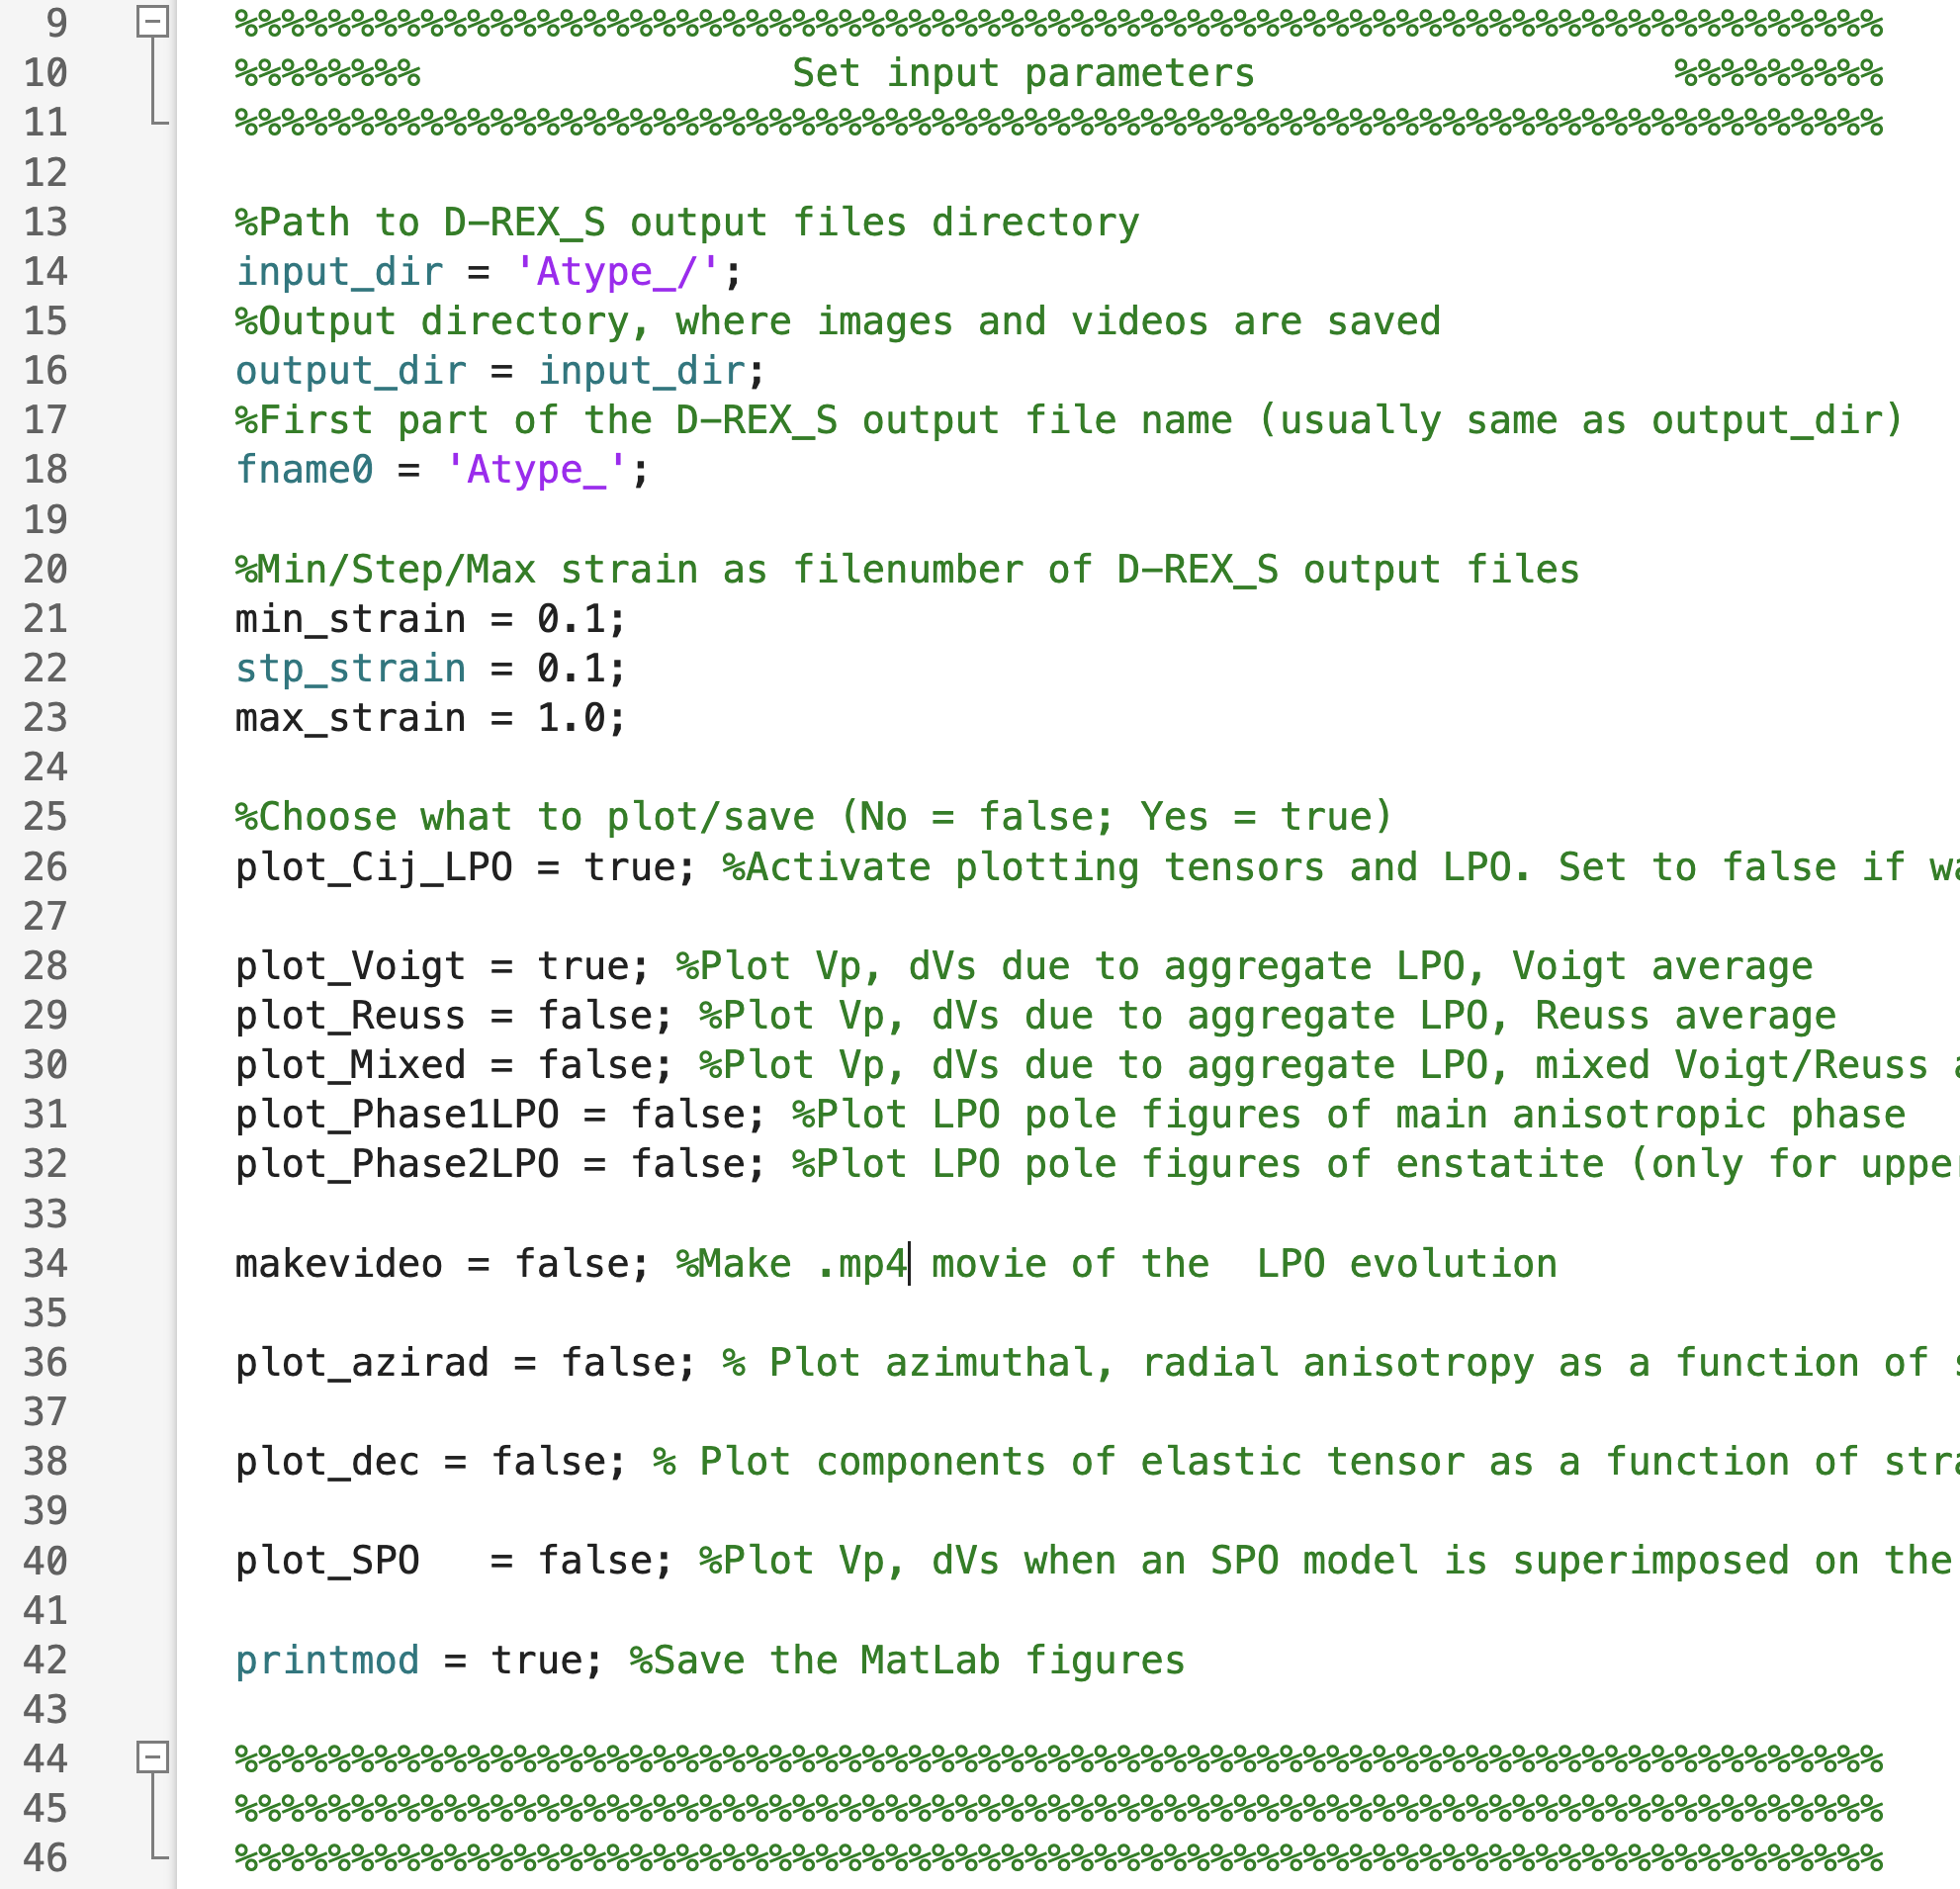
\includegraphics[width=1.0\textwidth]{DREX_S/drexs_viz.png}
    \caption{Control parameters in \texttt{read\_Cij\_LPO.m} for visualizing the \drexstitle{} output. In this particular case: generate pole figures of Vp, Vs1 and dVs for the elastic tensor obtained with the Voigt averaging scheme.}
    \label{fig:drexs_viz}
\end{figure}

\begin{figure}[ht]
    \centering
    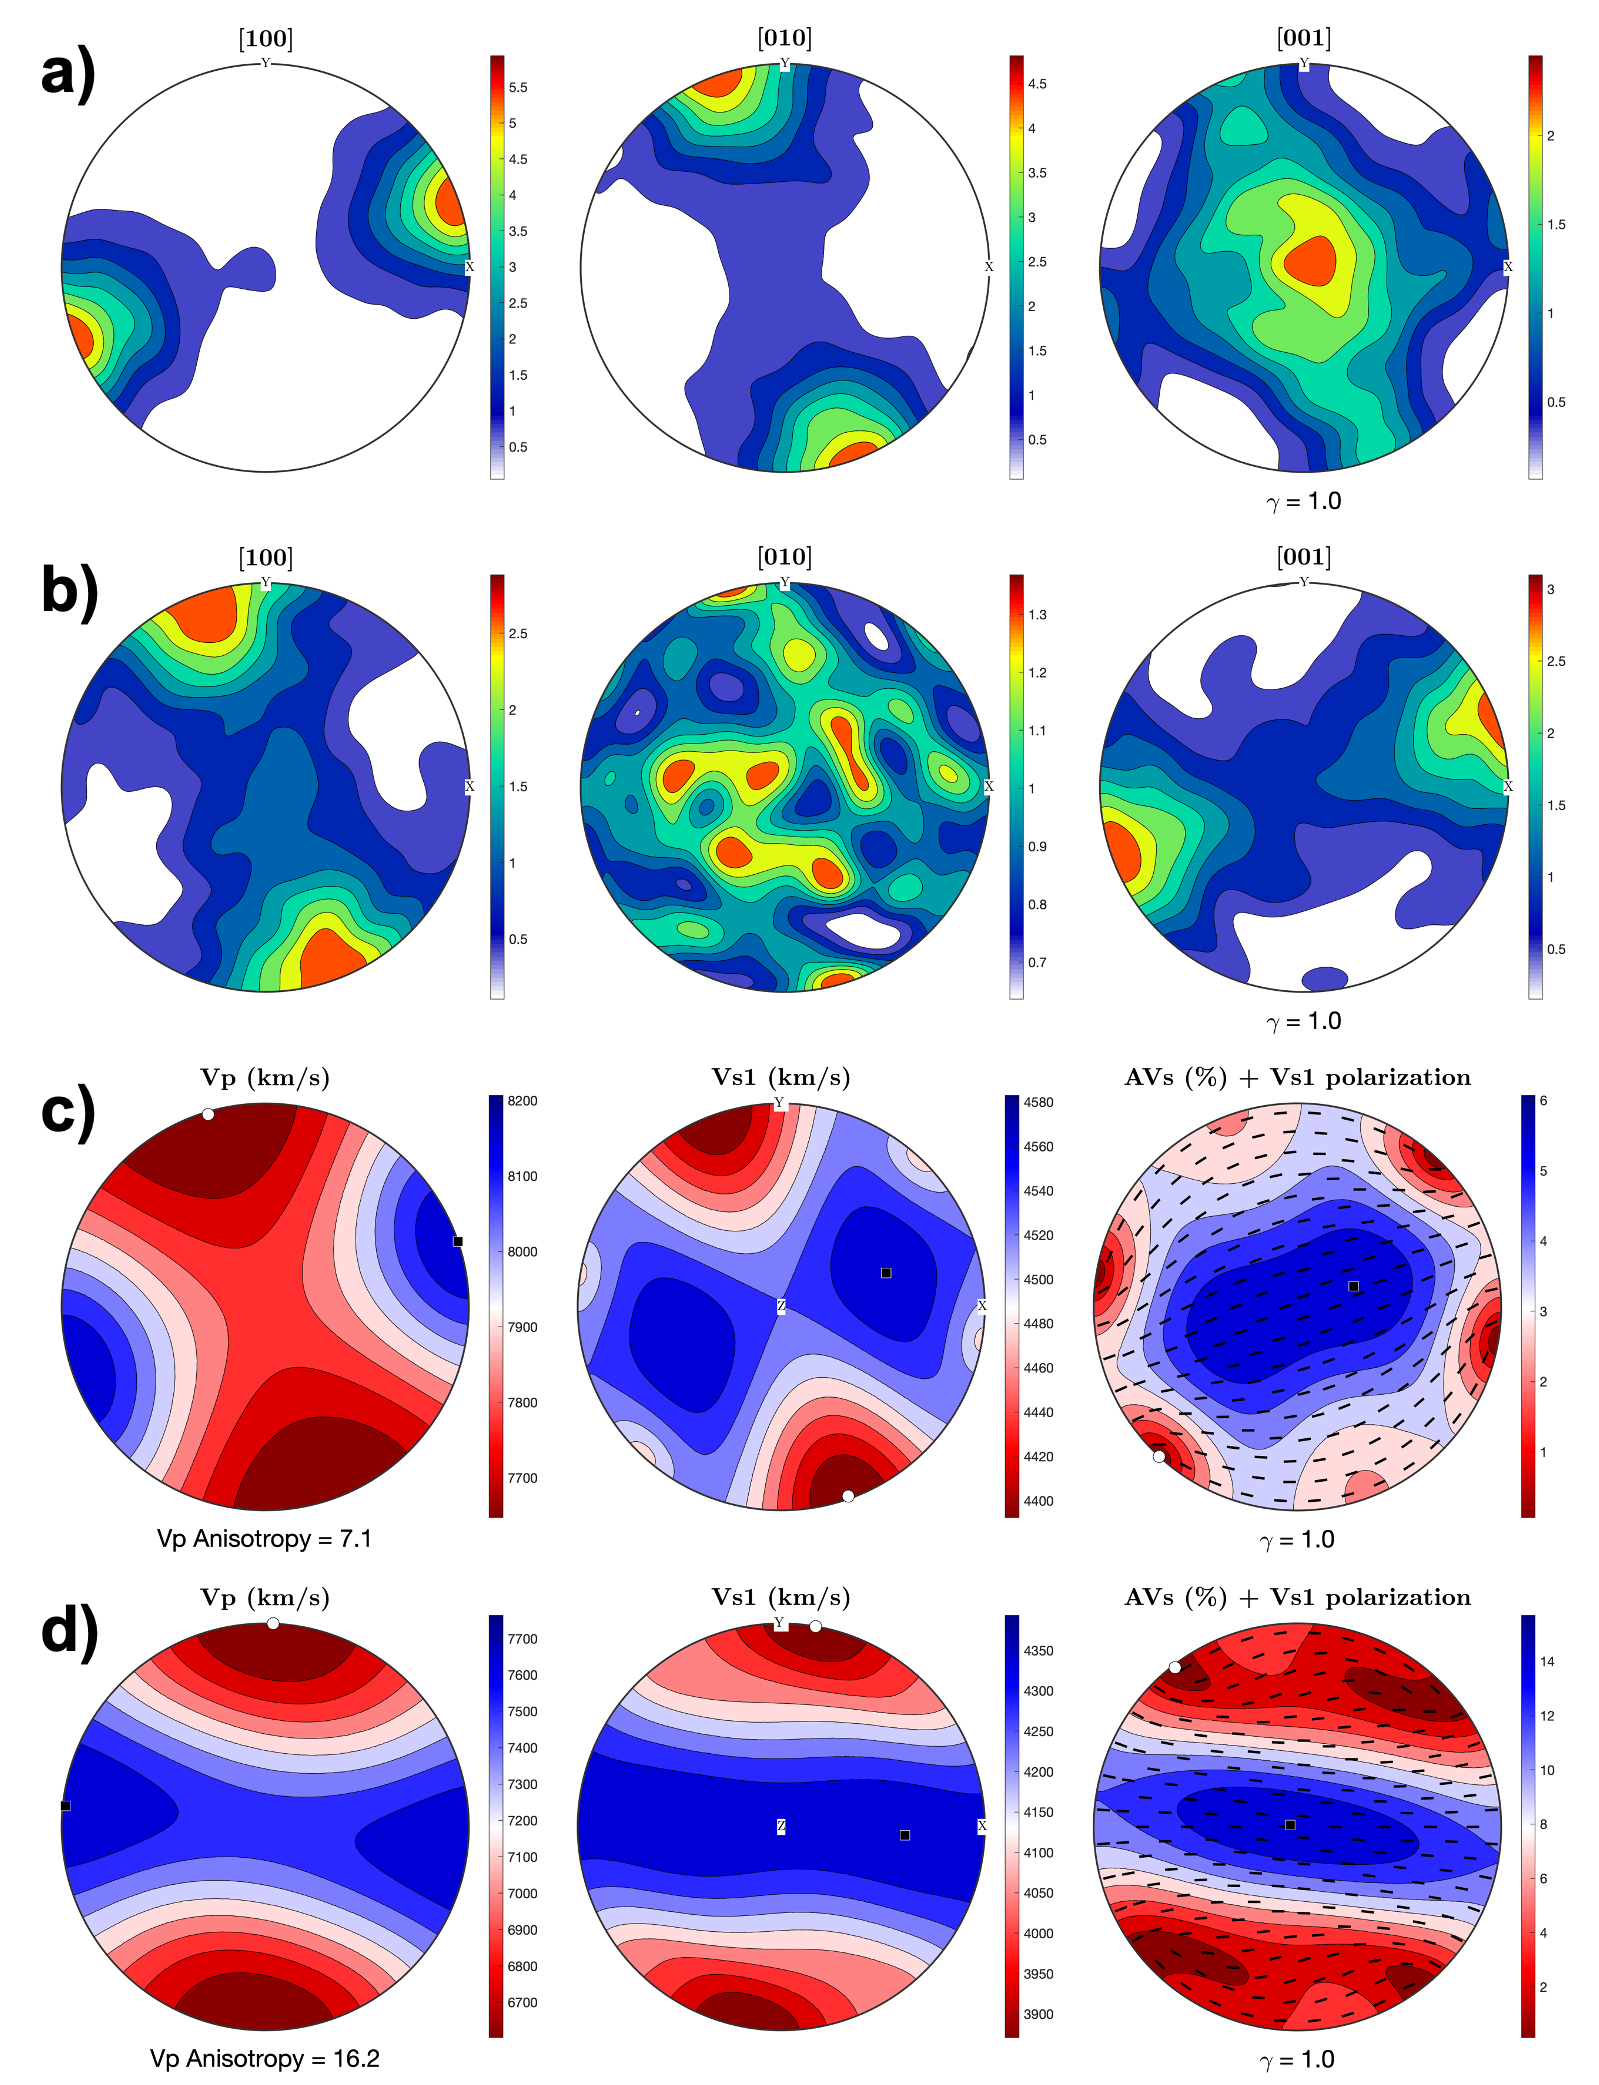
\includegraphics[width=1.0\textwidth]{DREX_S/Atype_summary_manual.png}
    \caption{Example of UM fabric after right-lateral simple shear strain of 1.0 with Ol:Ens = 70:30, \fonts{Mob} = 10, $\pmb{\lambda}=5$, $\pmb{\chi}=0.3$. (A) Olivine (A-type) LPO; (B) Enstatite LPO; (C) Vp, Vs1, and dVs + polarization direction of the fast shear wave component for the Mixed (Hill average) elastic tensor  resulting from the LPO fabrics in (A) and (B); (D) same as (C) but with superimposed an SPO fabric due to 5\% of melt-filled inclusions (10:10:1) oriented at -30$^{\circ}$ from the principal stress axis (which is at 45$^{\circ}$ from the horizontal plane).}
    \label{fig:atype}
\end{figure}

\begin{figure}[ht]
    \centering
    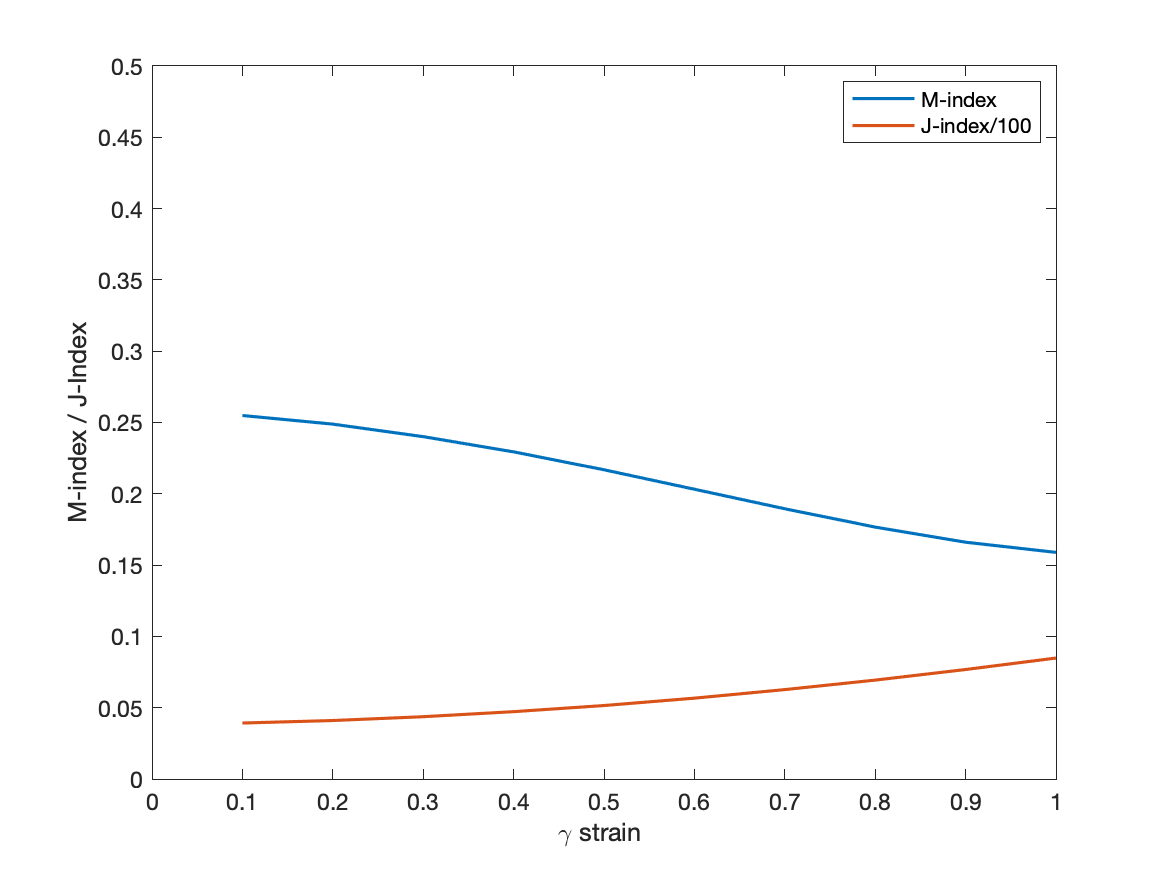
\includegraphics[width=1.0\textwidth]{DREX_S/MI_JI_Atype_.png}
    \caption{Evolution of M-index and J-index for an A-type olivine fabric.}
    \label{fig:miji}
\end{figure}

\begin{figure}[ht]
    \centering
    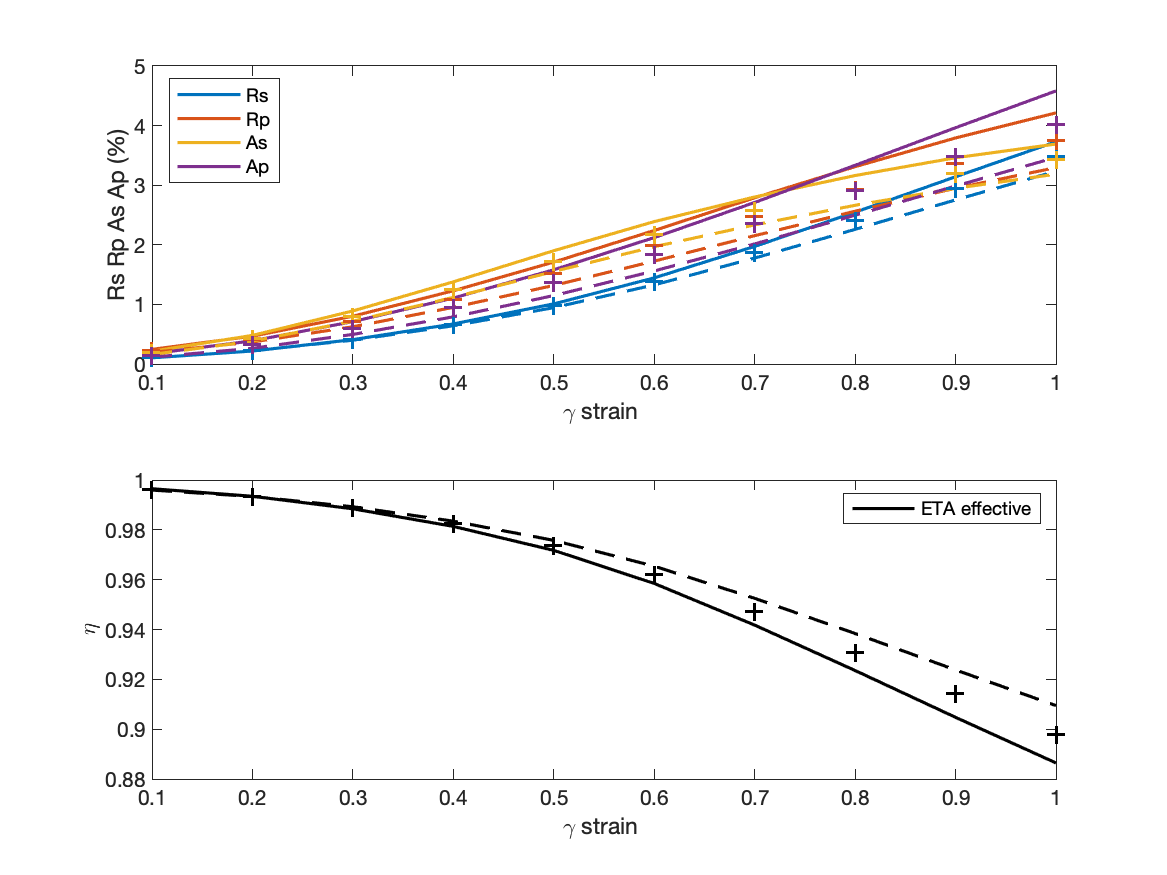
\includegraphics[width=1.0\textwidth]{DREX_S/AziRad.png}
    \caption{Evolution of radial and azimuthal P and S-wave anisotropy, and $\eta$ parameter for Voigt (continuous lines), Reuss (dashed lines) and Hill (+ symbols) averages.}
    \label{fig:azirad}
\end{figure}

\begin{figure}[ht]
    \centering
    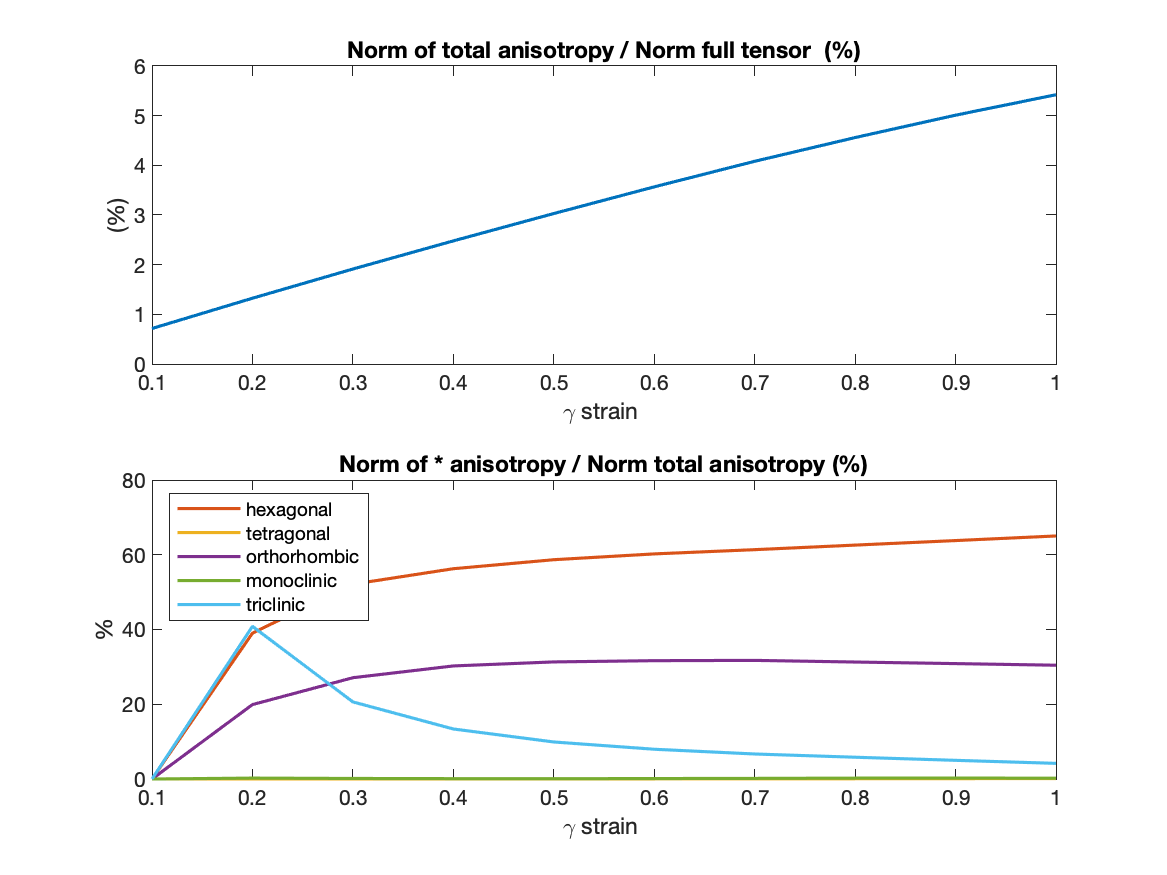
\includegraphics[width=1.0\textwidth]{DREX_S/dec.png}
    \caption{Evolution of (top) the norm of the total anisotropy component of the tensor over the norm of the full tensor (in \%), and (bottom) the norm of each anisotropic component of the tensor normalized over the norm of the total anisotropic component (in \%), computed for the elastic tensor obtained with the Mixed average.}
    \label{fig:dec}
\end{figure}

\vfill % Fill the rest of the page with whitespace